\chapter{System Design}
\label{chp:design}

% section overview, main components. Libtorrent as dependency. 
The goal in this thesis is to implement and evaluate a system where it can be used to both invest credit and improve swarm performance. In this thesis, we introduce ``Credit mining system'', an automatic investment framework on swarm with multidimensional gain. With credit mining system, locally, a user can gain credit with internally limited bandwidth allocation without any intervention needed. The credit can be in many forms such as share ratio (upload-to-download ratio), uploaded amount, effort based credit, and many other. From higher perspective, credit mining system will help a swarm to keep alive by providing integral pieces to the peer who need it. Although credit mining system will be implemented in Tribler system, it is possible to apply this feature to any file-sharing system.

In this chapter, the design of credit mining system is presented. This system consists of several subroutines which will be explained afterwards in section \ref{section:cmcomponents}. Under Tribler implementation, credit mining system heavily relied on \texttt{share mode} module of \textit{libtorrent}. \texttt{Share mode} is a module which can be activated as an intent to helping a swarm instead of normal content downloading. This module will be explained in detail in section \ref{section:sharemode}. The rest of the section \ref{section:libtorrent} explain other relevant, yet important module that credit mining system can exploit.

\section{Credit Mining Main Components}
\label{section:cmcomponents}

Credit mining system is intended to do its task automatically with minimal user intervention. The way this system designed is to align supply and demand of chosen swarm. Short term advantage of this approach is to gain credit by minimal download and maximize upload. In the long term, this potentially increase overall performance of other user as well.

The system can be implemented beside any torrent client. In Figure \ref{fig:cmcomponents}, it shown the compulsory elements and the relation between \textit{credit mining system} and \textit{torrent client}. Currently, we assume that every torrent client also track how much data a user has been downloaded and uploaded. We called this tracking history as \textit{credit storage} or \textit{bank}. Naturally, any torrent client must have \textit{downloading module} as well. Other dependency are te \textit{libtorrent} library. Credit mining system will use some of the \textit{libtorrent}-specific function. This function is not part of the \bt~Enhancement Protocol (BEP) which define the standard of \bt~protocol that need to be implemented. Other required feature is the ability of discovering peer by all method (DHT, PEX, LSD, etc). In some cases, peer discovery function is disabled for security reasons. While disabling one should not affect credit mining system, it will reduce the prediction and overall performance.

Credit mining system consists of several elements. First is the \textit{credit mining manager}. The \textit{manager} receives the \textit{settings} from user in the initial phase. To control mining process, user can only interact with value at \textit{settings} elements. User also limited to only add and remove \textit{mining source}. Each of the source will be assigned with a \textit{miner} depend on the type of the source. Miner also has sub-elements as part of the system. In-depth explanation of mining source and miners will be discussed in Section \ref{section:msource}. We introduce the \textit{predownload} mechanism as a way to evaluate a source early. This mechanism is launched by the manager instead of miner as it only happen during \textit{early propecting stage}. Predownload mechanism and prospecting methodology in general will be discussed in Section \ref{section:prospection}.

\begin{figure}[ht]
	\centering
	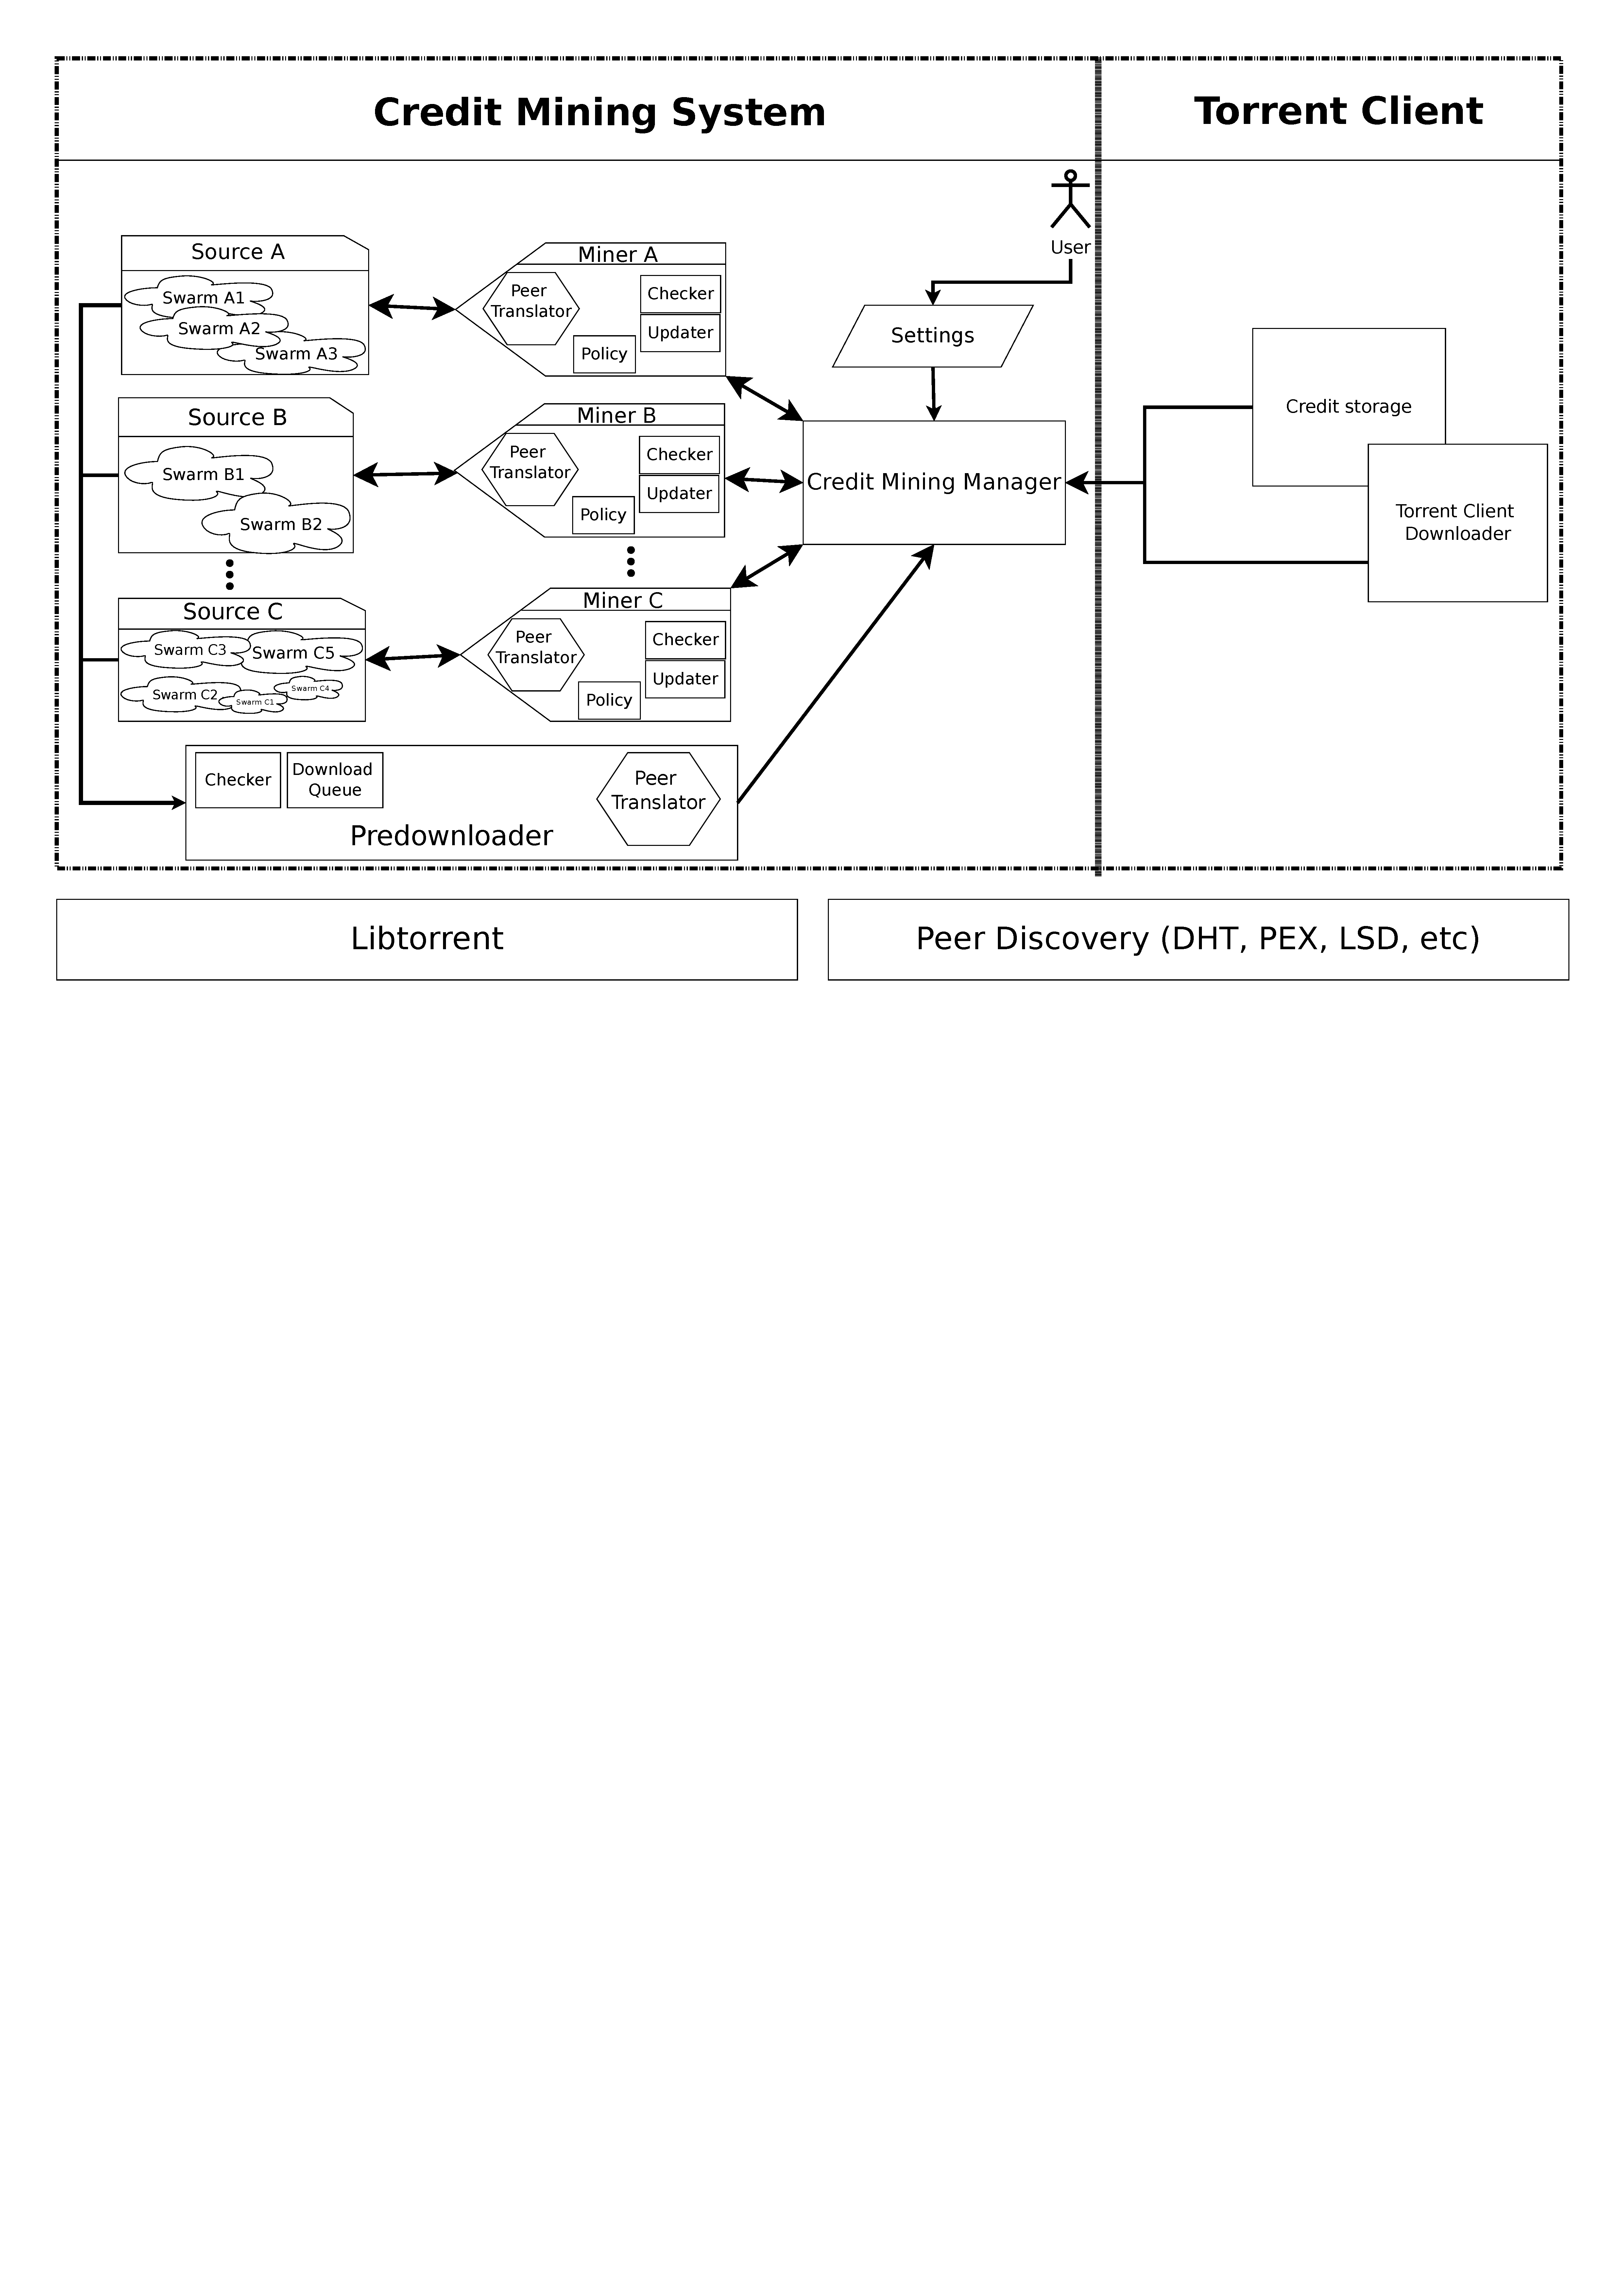
\includegraphics[width=\textwidth]{pics/cm_components.pdf}
	\caption{Credit mining components.}
	\label{fig:cmcomponents}
\end{figure}

% general flow
First, user can change the default settings used in the credit mining system. Some can not be changed when its already running. Table \ref{tbl:cmsettings} shows the settings used in this system. 

\begin{table}[]
	\centering
	\caption{Credit mining settings}
	\label{tbl:cmsettings}
	\begin{adjustwidth}{-1.5cm}{}
	\begin{tabular}{|p{1cm}|p{4cm}|p{7cm}|p{2cm}|}
		\hline
		\rowcolor[HTML]{EFEFEF} 
		No. & Name & Description & Changeable at runtime \\ \hline
	1 & \textit{max\_torrents\_active} & The maximum number of simultaneous swarm that will be downloaded & Yes \\ \hline
	2 & \textit{max\_torrents\_per\_source} & The maximum number of stored torrent in a miner that will be considered for mining & Yes \\ \hline
	3 & \textit{source\_interval} & The interval needed to check for updates in the swarm & Yes \\ \hline
	4 & \textit{swarm\_interval} & The interval to re-evaluate swarm and start/stop swarm & Yes \\ \hline
	5 & \textit{share\_mode\_target} & Libtorrent share mode target (See Section \ref{section:sharemode}) & No \\ \hline
	6 & \textit{policy} & The policy used in mining (See Section \ref{section:prospection}) & No \\ \hline
	7 & \textit{logging\_interval} & The interval for logging, for debugging purpose & No \\ \hline
	8 & \textit{tracker\_interval} & The interval to check for a new peer by peer discovery methods & No \\ \hline
	9 & \textit{timeout\_torrent\_activity} & The maximum time threshold to mark a swarm as 'inactive' & Yes \\ \hline
	\end{tabular}
	\end{adjustwidth}
\end{table}

\subsection{Mining Sources}
\label{section:msource} 
Currently, credit mining can accommodate three types of sources. There are directory source, RSS source, and channel source. In credit mining system, one source is assigned to one miner. The miner will start working the moment the source is defined and added to the manager. A miner periodically perform checking and other operations on all the torrents in the source. The operation that run in specified interval implemented differently for each of the source type. 

First type of source which called \textit{directory source}, is very straightforward. It takes a path as an argument and verify it before run the miner. The miner starts by looking at all the file in specified directory that have \texttt{.torrent} file type. Each of the file is examined and validated. Corrupt or invalid file will be discarded and deleted automatically from the disk. To keep the performance and prevent disk bottleneck, the miner sort the files alphabetically and put it into queue one by one. Miner periodically monitor both the directory if there is a new file and the queue to assign it to the manager. Miner eventually will pop an item from the queue, build a suitable format for mining, and notify manager to include this swarm.

Next possible mining source is from RSS (Rich Site Summary). RSS is a well known method to fetch new published data from a web. An RSS document contains the list of affected content which usually has summarized text and metadata. XML (Extensible Markup Language) format is widely used in RSS because of its compatibility and efficient size. An RSS from torrent portal such as etree\footnote{\url{http://bt.etree.org/rss/bt_etree_org.rdf}} and mininova\footnote{\url{http://www.mininova.org/rss.xml}} usually have title, publication date and a link to the swarm. Some mention number of seeder and leecher in the document. We called a source of RSS document as \textit{RSS feed}. 

In \textit{RSS source}, we assume that the RSS link user provided is available. If by any case the retrieval of the content is failed, the miner will stop immediately, notify the manager to disable this source, and shutting down itself. If the initial content retrieval is success, update mechanism will be launched periodically. In this mechanism, miner will fetch newest content from RSS feed. This content then parsed, resulting a list of swarm link and its metadata. Miner then asynchronously download the complete swarm data either via \texttt{.torrent} or magnet link. The same link will not be downloaded twice. After fetching the data, miner will build a defined format for mining, and notify manager to include this swarm. This data held across session. That means, another miner also will not download this swarm data in case it is indexed by other RSS feed.

\textit{Channel source} is the last type of source which tightly related to Tribler environment. As mentioned in section \ref{section:tribler} (Table \ref{tbl:community}), channel is responsible for managing torrents and playlists in Tribler community. A single channel can be discovered in \textit{AllChannel} community. Channel is identified by unique 40-length hexadecimal string. Naturally, Tribler user can create their own channel, put torrents into the channel, and share to other user. It is also possible for user to add a torrent to another user's channel. When a user subscribe to a channel, they will be notified if new torrent is added into that channel. Moreover, the torrents will be automatically downloaded into Tribler's database.

The flow of channel source is quite different with other type of source. It is tailored to follow Tribler specification which can change in the near future. Provided the identifier of a channel, miner will continuously try to find and join the channel in \textit{AllChannel}. By joined the channel, miner can get the list of torrents and other of its properties. After miner joined the channel, the swarm information will be handled and downloaded by Tribler. What miner do is to monitor the local database whether a new data has been fetched and there is a space for adding possible new torrent to the manager. Providing the swarm information, miner will download the \texttt{.torrent} file. It can be downloaded by using several options such as DHT, magnet link, or download from Tribler peers using TFTP (Trivial File Transfer Protocol). Downloaded \texttt{.torrent} will be stored in Tribler database. Afterwards, the mining format will be built and manager will be notified of a ready swarm.  

\subsection{Prospecting Methodology}
\label{section:prospection}
Prospecting a swarm is one of the key elements of credit mining system. The prospecting module can be divided into two main stage, named early and live prospecting. Both of the stages rely on the swarm measurement by looking at its evolution \cite{2013:swarmevolution:su}. 

Early prospecting stage is important to decide which swarm that need to be mined. Wrong or sub-optimal decision will lead to low credit to be mined and less effect on the swarm. In a case where the miner decide to choose a particular swarm, then it will optimistically find more information before it switch to another swarm if the decision is not beneficial. This will result with an unnecessary overhead on the miners as a whole.  

The challenge of early prospecting is because we only have very limited, unverified, information of the swarm. In the \bt~nature, there are two ways to get the swarm information : by joining the swarm as peer, or acting as a tracker. Mindlessly download and participate in the swarm may waste the resource we have. Therefore, in the manager, we proposed the procedure called \textit{predownloading}. On top of that, to both tackle the tracker unavailability and get thorough swarm information, \textit{peer translation} mechanism can act as a swarm health predictor.

\begin{algorithm}[h]
	\caption{\textit{Predownload} procedures}
	\label{alg:predown}
	\begin{algorithmic}[1]
		\Function{Predownload}{$infohash$, $n$}
		\If{$|download\_queue| > $ 500}	
		\State recall \Call{PREDOWNLOAD}{$infohash$, $n$}
		\EndIf
		
		\State \Call{push}{$download\_queue$, $infohash$}
		
		\State \Call{set\_pieces}{$infohash$, 0, $n$}
		\State \Call{unset\_pieces}{$infohash$, $n + 1$, \Call{pieces}{$infohash$}}
		
		\State \Call{check\_predownload}{$infohash$}
		\EndFunction
		\Statex
		\Function{check\_predownload}{$infohash$}
		\State $peerlist \gets$ \Call{get\_peers}{$infohash$}
		\State \Call{add\_to\_peerlib}{$peerlist$}
		
		\If{wait long enough $and$ not finished yet}
		\State \Call{pop}{$download\_queue$, $infohash$}
		\State \Return False
		\EndIf
		
		\If{wait long enough $and$ already finished}
		\State \Call{translate\_peer}{\Call{get\_peerlib}{\null}}
		\State \Call{pop}{$download\_queue$, $infohash$}
		\State \Return True
		\EndIf
		
		\If{\Call{is\_complete}{$infohash$}}
		\State mark as finished
		\EndIf
		\State \Call{check\_predownload}{$infohash$}
		\EndFunction		
	\end{algorithmic}
\end{algorithm}

\textit{Predownloading} is a means to download a predefined number of pieces in a particular torrent in such a way that only consumes small portion of resource while trying to get as much information as possible of the swarm. \textit{Predownloading} can run in a different session than the main one so it will not disturb the activity of the main session. Assuming we have $n$ piece to \textit{predownload}. The manager then will just explicitly download the first $n$ piece of a verified torrent and flag it as sequential download activity while reject the rest of the pieces. In this way, instead of occupying a large portion of storage, it only stores those $n$ pieces. While and after \textit{predownloading}, the manager actively ask for new peers to tracker or DHT and store it afterwards. There is a delay introduced when the manager has finished \textit{predownload} all those $n$ pieces. This delay is necessary to give a chance for another peer to response to the manager's query and to request new peer if possible. Pseudocode of this procedures shown in Algorithm \ref{alg:predown}. The mining activity will continue at the point where \textit{predownloading} finished. It will not restart the download from scratch.

To be able to fully decentralized, it is important to not rely on the tracker too much. Although some information we needed can be gathered by querying the tracker, some of the swarms don't have tracker at all. Furthermore, in case of multi-tracker\footnote{Defined in : \url{http://www.bittorrent.org/beps/bep_0012.html}.}, some swarms has entirely different number of seeder and peers for each of the tracker. In figure \ref{fig:diffsr}, it is shown that this problem is very likely to be occurred. Because of this reason, we alternate the swarm information source by looking directly from the connected peers. We called the procedure to interpret swarm information from current and previous connected peers as \textit{peer translating}. 

\begin{figure}[ht]
	\centering
	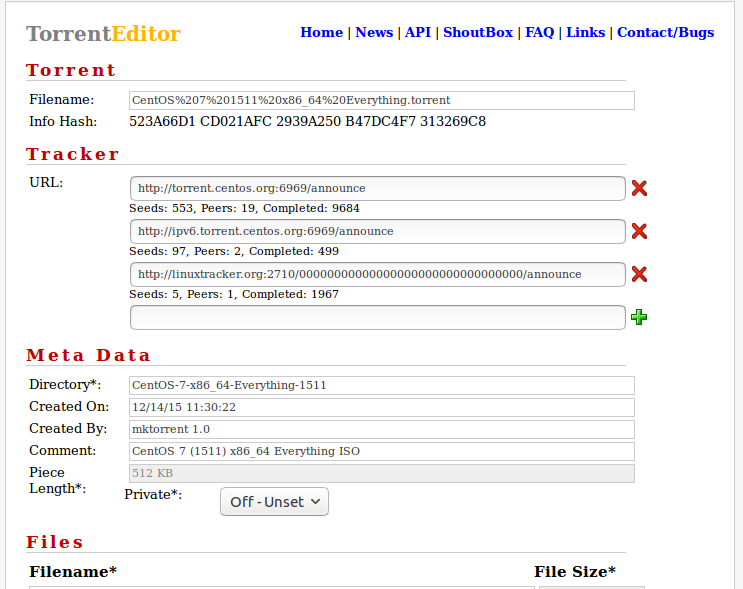
\includegraphics[width=0.8\textwidth]{pics/diffsr.png}
	\caption{Different number of seeder and peers/leecher reported by different trackers.}
	\label{fig:diffsr}
\end{figure}

The \textit{peer translation} receives list of peers as input and returns the number of seeder and downloader. This procedure is shown in Algorithm \ref{alg:peertrans1} and \ref{alg:peertrans2}. The manager will examine each of the peer like shown in \ref{alg:peertrans1}. We categorize a peer is seeder if it satisfy at least one of three conditions. The conditions are: it is only want to upload right now, it is 80\% finished with its download, and it is known to upload more data to us than downloading. In the other hand, we define a peer is a leecher if it satisfies at least one of three conditions, which is: it is interested in our pieces, it has unfinished download and able to download again another piece, and it is known to download more data from us than uploading. We called the phase where the analyzed peers are translated into number of potential seeder and leecher as \textit{interpretation} phase. This phase shown in Algorithm \ref{alg:peertrans2} which is the continuation of Algorithm \ref{alg:peertrans1}.

\begin{algorithm}[]
	\caption{Peer translation algorithm, analyzing phase}
	\label{alg:peertrans1}
	\begin{algorithmic}[1]
	\Function{translate\_peer}{$peer\_list$}
		\State{$num\_seeder \gets 0$}
		\State{$num\_leecher \gets 0$}
		\Statex
		\State{$upload\_only \gets 0$}
		\State{$finished \gets 0$}
		\State{$unfinished\_able \gets 0$}
		\State{$interested \gets 0$}
		\ForAll{$p \in peer\_list$}
			\If{\Call{upload\_only}{p}}	
			\State $upload\_only \gets upload\_only + 1$
			\EndIf	
			
			\If{\Call{interested}{p}}	
			\State $interested \gets interested + 1$
			\EndIf	
			
			\If{\Call{completed}{p} $>$ 80\%}	
			\State $finished \gets finished + 1$
			\Else
			\If{not \Call{upload\_only}{p}}	
			\State $unfinished\_able \gets unfinished\_able + 1$
			\EndIf	
			\EndIf
		\EndFor
		\algstore{peertranslate}
	\end{algorithmic}
\end{algorithm}

\begin{algorithm}[]
	\caption{Peer translation algorithm, interpretation phase}
	\label{alg:peertrans2}
	\begin{algorithmic}[1]
		\algrestore{peertranslate}
		\State $num\_seeder \gets $ \Call{max}{$upload\_only$, $finished$}
		\If{$num\_seeder = 0$}	
		\State $num\_seeder \gets $ number of peer who has downloaded bytes $>$ uploaded bytes
		\EndIf
		\State $num\_leecher \gets $ \Call{max}{$interested$, \Call{min}{$unfinished\_able$, $|peer\_list|$ - $finished$}}
		\If{$num\_leecher = 0$}	
		\State $num\_leecher \gets $ number of peer who has uploaded bytes $>$ downloaded bytes
		\EndIf
		\State \Return $num\_seeder$, $num\_leecher$
	\EndFunction
	\end{algorithmic}
\end{algorithm}

After the early prospecting has been done, the live prospecting stage will take place regularly. For a fixed interval, the manager will evaluate the miner performance. Each miner will have to choose which swarm to mine and to stop based on defined policy. We called this stage as \textit{swarm selection}. All the miner need to comply to one defined policy. 

\subsubsection{Swarm Selection}
Although it is possible for user to create their own policy, three policies have been defined on the preliminary work \cite{2015:creditmining:capota}. Those are based on random, swarm age, and seeder ratio. \textit{Random policy} mostly used as the baseline of the experiment. It is also able to stress test the miners. \textit{Swarm Age policy} is better than random policy. It selects the swarm based on its age. New published swarm known to have higher demand than other type of swarm \cite{2012:economicbt:kash}. Typical user will download a particular item once. Enthusiastic user will download a content as soon as it is published. With a lot of peer in early swarm, it will increase the chance to get more credit. \textit{Seeder Ratio policy} selects the swarm that has lower number of seeder relative to all the peers participated in this swarm. This policy is specialized to help undersupplied swarm. 

In this thesis, we intend to extend those policies so it can be highly customizable and cover the balance between gaining credit and helping undersupplied swarm. We propose a policy named \textit{scoring policy} to tackle this issue. Although this policy is more complex than the other basic policies, it is can be customize with several parameters and multipliers of the score. The algorithm of this policy is shown on Algorithm \ref{alg:scorep}. The idea behind this policy is to give higher score for swarm which has lower seeder ratio, has more peers, lower piece availability, and many activities in the swarm. Higher score get higher priority to be mined.

Lower seeder ratio, as mentioned before, is useful to measure whether a swarm is undersupplied or not. This is particularly useful to \textit{help} a swarm. However, in small swarm, this attribute may not be relevant. Thus, a number of peer is considered as a scoring aspect. With the same ratio of seeder and peers, it is useful to mine a big swarm instead of the small one. There are many options to give our piece to. Another important aspect is the file availability of the swarm. In flashcrowd case, there are a significant amount of peer who do not have a large portion of the file. Comparing to another swarm which most of the leecher almost finished their download, mining this swarm will give higher credit and more beneficial to the community altogether. Last element that we considered is the activity of a swarm. It is preferable to mine a swarm whose some of the peers already download or upload any data from or to us. The reason behind this is because the underlying nature of \bt, it is possible that our prediction is wrong. The worst case happened when there are no peer interested with the piece we already have. In the other hand, if a peer already interacted with us before, there is a chance we will get chosen again in the future. Therefore, by putting this attribute into consideration, we want to minimize this problem.

\begin{algorithm}[h]
	\caption{Scoring policy algorithm}
	\label{alg:scorep}
	\begin{algorithmic}[1]
		\Require{$M\_leech$ as leecher multiplier}
		\Require{$M\_pratio$ as peer ratio multiplier}
		\Require{$M\_avail$ as peer availability multiplier}
		\Require{$S\_low$ as score for lower activity}
		\Require{$S\_high$ as score for higher activity}
		\Statex
		\Require{$peerlist$}
		\Require{$swarmlist$}
		\Statex
		\ForAll{$s \in swarmlist$}
			\State{$rleech \gets 1 - $\Call{seeder\_ratio}{s}}
			\State{$rpeer \gets |$\Call{peers}{s}$|/|peerlist|$}
			\State{$ravail \gets 1 - $\Call{availability}{s}$/|peerlist|$}
			\State{$score(s) \gets M\_leech*rleech + M\_pratio * rpeer + M\_avail * ravail$}			\State $total\_speed[s] \gets 0$
			\ForAll{$p \in $\Call{peers}{$s$}}
				\State $total\_speed[s] \gets total\_speed[s] + speed(p)$
			\EndFor
		\EndFor
		\State \Call{sort}{$total\_speed$}
		\ForAll{$s \in swarmlist$}
			\If{$index(total\_speed, s) < |total\_speed|/2$}
				\State $score(s) \gets score(s) + S\_low$
			\Else{\null}
				\State $score(s) \gets score(s) + S\_high$
			\EndIf
		\EndFor
		\State \Return{$score(swarmlist)$}
	\end{algorithmic}
\end{algorithm}

Scoring policy starts with examining all the swarm in a particular miner. Then we decide the score individually as shown in line 2-5. \textit{Peer ratio} is the ratio of a number of peer in this swarm and total number of peers that we know from all the swarm. \textit{Availability} is defined as the number of complete copies of a piece. Non-seeder peer provide a subset of a piece and increase the overall of the availability. In this case, we add the \textit{availability} as the number of peer who has the rarest piece. Moreover, the fraction of piece who has more peer is also considered. It is impossible for \textit{availability} to be 0, as it means there is no one who have complete file. Maximum number of \textit{availability} is the number of peer itself. That means, all the peer has completed files. After the score was assigned, the activity of each peer on each of the swarm is calculated. The activity, stored in a list, is sorted increasingly. Then, first half of the sorted activity is marked as low activity, and given the lower activity score (line 14). Similarly happens with second half of the list, but with higher activity and higher score (line 16).

\subsection{Resource Optimization}
\begin{itemize}
	\item starvation prevention, no immediate stopping
	 \item fallback mechanism (for now)
\item 	 swarm blacklisting
\item 	 resume downloading (cache)
\item 	 archival mode
\end{itemize}


\section{Libtorrent}
\label{section:libtorrent}
Another Tribler dependency is \textit{libtorrent}\footnote{\url{http://libtorrent.org/}}. With \bt~is just a collection of specification, it free to be implemented with any languages. One of the implementation in \texttt{C++} is \textit{libtorrent}. \textit{libtorrent} also has \texttt{python} binding which the same language as Tribler implementation. \textit{Libtorrent} started in 2003 by Arvid Norberg. \textit{Libtorrent} is used by many torrent client such as Deluge, qBittorrent, Free download managers, and many others.

\subsection{Piece picker control}

\subsection{Priority Management}
priority in libtorrent. Unchoke round. Bandwidth control

\subsection{Share Mode}
\label{section:sharemode}
One of the crucial feature used in this work is \textit{share mode} \footnote{Core code of share mode can be found in \url{https://github.com/arvidn/libtorrent/blob/master/src/torrent.cpp\#L9586-L9727}}. Initial work performed by \citeauthor{2015:creditmining:capota} also used this feature\cite{2015:creditmining:capota}. By enabling share mode, it means that one is not interested in downloading the file, but gaining higher share ratio. It is done by download as little as possible and upload as much as possible. Share mode only download a torrent where it has sufficient capacity. A torrent downloaded in share mode may never finish as \textit{libtorrent} only download piece of a torrent which satisfied the share mode requirements. Share mode can be enabled per torrent basis.

Share mode algorithm works heuristically as it estimates the rarest piece available in the swarm based on participated peers. First, it tries to find whether there is a piece which nobody has (line \ref{alg:l_lts:missingp}). Note that in line \ref{alg:l_lts:disconnectpeers}, libtorrent disconnect some of the seeder because we need to connect to the leecher later. This case is considered if there are too many seeder in our connection pool. Next, the number of missing pieces is decreased linearly with the number of seeder. This is based on assumption that both of us and other seeder can upload at least one piece each (line \ref{alg:l_lts:reducemissing}). To keep the performance, downloading piece activity is stacked until more than 5\% of the number to be downloaded (line \ref{alg:l_lts:retdling}). To determine rarest piece, libtorrent count the number of peer that has that piece. The number of peer on the rarest piece is termed \textit{rarity}. Share mode ensure that we only download the rarest piece available in the network (line \ref{alg:l_lts:rarepc}). We end the prematurely routine if there are more number of piece to download compared to uploaded (line \ref{alg:l_lts:retdlenough}) or there are not enough peer to upload the rarest piece (line \ref{alg:l_lts:rareunable}). Both condition will prevent us to get positive share ratio. Finally, it will download randomly the rarest pieces if there are more than one option (line \ref{alg:l_lts:dlrare}). The algorithm presented in algorithm \ref{alg:ltsharemode}. 

\begin{algorithm}[]
	\caption{Libtorrent share mode algorithm}
	\label{alg:ltsharemode}
	\begin{algorithmic}[1]
		\Require{$T$ as share mode target}
		\Statex
		\State{$missing\_piece = 0$}
		\ForAll{$p \in connected\_peers$}
		\If{$p$ is a $leecher$ $and$ $p$ is not in share\_mode}	
		\State{$missing\_pieces$} += {$total\_pieces - pieces(p)$} \label{alg:l_lts:missingp}
		\EndIf	
		\EndFor
		\If{$|connected\_seeders|$ in $connected\_peer$ $>$ $90\%$}	
		\State disconnect excess seeder \label{alg:l_lts:disconnectpeers}
		\EndIf
		\State{$missing\_pieces$} -= {$2 \times |connected\_seeders|$}	\label{alg:l_lts:reducemissing}	
		\If{$missing\_pieces \leq 0$}
		\State \Return
		\EndIf
		\If{$num\_to\_downloaded \times T > uploaded$} \label{alg:l_lts:retdlenough}
		\State \Return
		\EndIf
		\If{$downloading < 5\% \times num\_to\_downloaded$} \label{alg:l_lts:retdling}
		\State \Return
		\EndIf
		\ForAll{$pc \in pieces()$}
		\If{$pc$ not in $collected\_piece$ $and$ $peer\_count(pc) \leq rarest\_rarity$ }	\label{alg:l_lts:rarepc}
		\State{$rarest\_rarity$} = {$peer\_count(pc)$} 
		\State{$rare\_piece$.push($pc$)}
		\EndIf	
		\EndFor
		\If{$|connected\_peers| - rarest\_rarity < T$} \label{alg:l_lts:rareunable}
		\State \Return
		\EndIf
		\State download {$random(rare\_piece)$} \label{alg:l_lts:dlrare}
	\end{algorithmic}
\end{algorithm}

There are several limitations on this feature as we observed. First, it only has single parameter which determine the desired target of share ratio. This limits the exploration and full use of share mode feature. Another issues are storage and network inefficiency. If enabled, share mode works by downloading popular piece of a particular torrent. This means few downloaded pieces could take a large storage. Share mode also did not check whether a swarm is efficient enough to perform this operation. It only tries to find popular pieces regardless of the swarm condition. It is highly possible that if a swarm is in poor capacity, the uploading rate is very low. The bandwidth used to check torrent pieces regularly is wasted and the ``investment'' will not go well.